\section{Computer Experiments} \label{ch:computer_experiments}

This section describes the setup and configuration of the computational experiments conducted in this study, and the accompanied results. Two types of statistical models, \acrshort{convlstm} and \acrshort{ar}-model are trained and evaluated on an unseen portion of the dataset. 

\subsection{Framework, Structure and Implementation} \label{sec:structure_and_implementations} \label{sec:framework}
%\section{Structure and Implementations} 
The numerical methods used in this study are described in Chapter \ref{ch:num_methods}. The code is available on GitHub in the project repository named ``MS'' on \href{https://github.com/hannasv/MS}{https://github.com/hannasv/MS}. Instructions for downloading 
reanalysis (ERA5) data using python is provided. 
The dataset is not published because of a licences on the \acrshort{msg} data. 
%Due to licence requirements on the \acrshort{msg} data, no part of \acrshort{ecc} is made available for downloading. %The reader need to aquire their own \acrshort{msg} data throught the eumetcast portal and can regridd the product using the code made availble.

%\textbf{Due to liscence on the MSG data in finer than X resolution, the full dataset is not made aailable. The code for regridding and thedescriptions for downloading the data is made available.}



%The repository contains everything need to reproduce the results in this study.
%The experiments are conducted in notebooks and the developed modules are stored in the package ``sciclouds''. Descriptions on how to acquire the data (scripts if possible) and project environment is provided to simplify the process.

The code is developed in Python 3.7, a popular language for scientific software development. The source code is stored in the package \textit{sciclouds}, made available on Github through the project repository. Developed modules draw inspiration from the structure of \textit{scikit-learn} (\cite{sklearn_api}).
%and the \textit{keras-tuner} (\cite{chollet2015kerastuner}). 
%The \acrshort{convlstm} is implemented %in \textit{keras} (\cite{chollet2015keras})
%using \textit{tensorflow v 2.0} . %The \textit{keras-tuner} is used to automize the hyperparameter search (\cite{chollet2015kerastuner}). 
The \acrshort{convlstm} is implemented using Tensorflow's keras API (\cite{tensorflow2015}) which simplifies many aspects of building and executing machine learning models. To utilize the analytical solution the \acrshort{ar}-models are trained and evaluated using self implemented modules.
%The \acrshort{ar}-models are trained and evaluated using self implemented modules. The idea was to utilize the analytical solution of the least squares problem. 
%Many regression modules provide a numerical solution, not the analytical. 
The python package ``sclouds'' provides a self implemented version of \acrshort{ar}-models, using the analytical solution to the least squares problem derived in Section \ref{sec:ARmodels}.

Visualizations are generated using \textit{Matplotlib} (\cite{matplotlib}),  \textit{Seaborn} (\cite{seaborn}) and maps using the package \textit{Cartopy} (\cite{Cartopy}). Other illustrations are developed using TIkZ, a language used for producing technical illustrations within the environment of LaTeX.

The package versions are documented in the \textit{requirements.txt} and the project environment called ``sciclouds'' is ready for installation. This is a conda environment, the yaml-file lists the Python packages and requirements necessary for running this code. Below you find the code example for cloning the project and installing the environment.

% Included in the readme file on github. 
\begin{verbatim}
git clone https://github.com/hannasv/MS.git
cd MS
conda env create -f environment.yml
conda activate sciclouds
python setup.py install # installing package from source
\end{verbatim}

Supplementary material for remapping satellite data and filtering masks is available in the supplementary repository \href{https://github.com/hannasv/MS-suppl}{https://github.com/hannasv/MS-suppl}. %To make use of all the functionality available trought ``MS'', the supplementary repository needs to be cloned in the same directory.
The filters are generated from within the environment of PyAEROCOM (\cite{pyaerocom}). 


%Complex computations will cause memory growth, dependant on how many intermediate computations it needs to store. This is the case for \acrshort{convlstm}. To speed up the development process the software is developed on a subset of \acrshort{ecc}. Small adjustments needs to be made, running experiments on the entire data. For instance threads deadlock when extracting large amounts of data. This is a precautionary measure to avoid overloading the system. \textbf{Possible to develop code to do Hyperparameter tuning based on }
%For a more detailed description please see the project repository described in Section \ref{sec:structure_and_implementations}.

\subsection{Hardware} \label{sec:hardware}
%How to deal with big datasets that will easily eat up you memory? ``Big data'' involve processing large amounts of data that does not fit into memory. Processing substantial amounts of data require expert knowledge about distributed systems and analysing for system bottlenecks.  %Although theoretically fascinating it remains to see if \acrshort{convlstm} provide a clear practical advantage over the autoregressive models.
%Conducting experiments on big datasets require external computational resources.  
The experiments described below, are conducted on a 
%This study had access to a 
DGX-2 system consisting of 16 NVIDIA Tesla V100 GPUs, each of 32Gb local memory and 1.5Tb shared memory. %The resources was available through the \acrfull{ex3} project hosted at Simula. 
%This study was awarded access to 1 GPU and 1024G part of the memory. 
The data is stored on a \acrfull{rdma} accessed over Infiniband. %\textit{The best choice of collective implementation depends upon the number and kind of \acrshort{gpu}s, and the network interconnect in the cluster.} 
The DGX-2 system is designed for a high level concurrency and scheduling workers competing for system resources.
%The hardware sets the limitations for efficiency of pipelines and training procedure. 
%\textit{NVIDIA V100 GPU -- The eX3 infrastructure includes a DGX-2 system consisting of 16 NVIDIA Tesla V100 GPUs, allowing simultaneous communication between all eight GPU pairs at 300 GBps through the 12 integrated NVSwitches. This gives a theoretical system-wide system bi-directional  bandwidth of 2.4 TBps. All GPUs have 32 GB of local memory (total of 512 GB) and share a 1.5 TB main memory. The total system has 81,920 CUDA cores, and 10,240 Tensor cores delivering 2 Petaflops of tensor performance. The peak performance in double precision is 125 Teraflops.}
%Working on such a monstrosity pose additional challenges related to porting existing code and virtual environments, developing and debugging code. To eventually end up with an%a achieved 
%acceptable level of efficiency and reliability. \textbf{må de siteres? (\cite{ex3docs} and \cite{ex3homepage}).} 
\begin{table}[ht]
    \centering
    \begin{tabular}{c|c}
        Device &  Type  \\ \hline
        GPU & Tesla V100-SXM3-32GB \\
        CPU & DualProcessor AMD Epyc7601 (SMT2) w/2TB ram and 4TB NVMe 
    \end{tabular}
    \caption{Hardware specifications for the environment used on \acrshort{ex3}. The operating system is Ubuntu 18.04.4.}
    \label{tab:hardware_ex3}
\end{table}
%\textbf{TS: Mye av teksten frem til dette punktet egner seg egentlig bedre i et Appendix}
%TS: Mye av teksten frem til dette punktet egner seg egentlig bedre i et Appendix
\subsection{Model Setup and Evaluation}
The following sections contain the configurations of the models compiled for this study. A configuration is a set of parameters set prior to training. These are often referred to as hyperparameters, as mentioned in Section \ref{sec:artificial neural networks}.

%A model is compiled based on a choice of hyperparameters. It is a set of decisions made prior to training, as mentioned in Section \ref{sec:artificial neural networks}.
In the search for the best model configuration, different combinations of hyperparameters are evaluated based on a metric. % mention why you chose M;A;E?
This study evaluate models based on \acrfull{mae}, see Section \ref{sec:metrics} for more details.

For the more complex \acrshort{dl}-models, the choice of architecture (model configuration) can easily overload the system memory resources. Therefore the tuning of \acrshort{convlstm}-models was done manually. There is a mind-boggling amount of choices for hyperparameters, the initial configuration used in the conducted experiments for this project draw inspiration from this paper by \citeauthor{SunAirLSTM} (\citeyear{SunAirLSTM}).
The models are described in Section \ref{sec:related_work}.
The \acrshort{ar}-models follow another strategy. For this study the simplest models was trained first, followed by a gradual increase in complexity.
%This could have been done using spaced sampling, attempting lags of 1, 2, 5, 10. The result becomes the same, however for large model there might be some time to save.

%it follows the principal of starting with the simplest model possible and increasing the complexity from there. 
%Stopping at architectures where increased complexity don't increase the performance? Know stategies are using spaced sampling, attempting lags of 1, 2, 5, 10. The second is naturally to further investigate regons of lags showing the most promise. 
%on a similar problem, air quality forecasting problem was executed. \citepaper{chollet2015kerastuner} provide suitable software for the automatic hyperparameter tuning. 
%\textbf{Man kjører eksperimenter på mange modeller ved å bruke traning og validations dataset. The choice of model is based on this data basis and then it performance is tested on the test dataset.} 
\subsection{Training, validation and test split}
Gradient methods are at the heart of every machine 
learning algorithms. This type of optimization is based on the principle that the model is continuously evaluated against the validation dataset and weights are adjusted to reduce the loss. This raises the need for two datasets during training. The \acrshort{ar}-models are computed based on an analytical solution and have no need for the extra data set. 

Based on the assumption that the most resent partition is representative for the near future, both models were tested on 2014 to 2018. The \acrshort{ar}-model is trained on the period 2004 to 2013, while the \acrshort{convlstm} is trained on  2004 to 2011 and validated on 2012 to 2013.

Other notable differences in the input data is related to handling missing values.  
%Missing data arise from failed retrivals. Consequently entire grids are missing and not individual pixels. 
The \acrshort{ar}-models use shorter sequences, and samples containing missing values are simply removed. The \acrshort{convlstm}-model utilize longer sequences, and missing values are replaced by the out-of-sample value, $c=1.5$. 

%The test period was chosen based on the assumption that the latest period is most representative for the climate in the near future. The handling \textbf{(nytt ord)} of gaps, provide an additional difference to the datasets used as input for the \acrshort{ar} and the \acrshort{convlstm}-models. The order of the \acrshort{ar}-model determines the length of the training sequence. All samples with gaps in the requested sequence are disregarded causing a reduction in the data basis for a model of a particular order, determined by the number of lags. For the \acrshort{convlstm} these gaps are filled with an out-of-sample value, $c=1.5$. 
\subsubsection{Autoregressive models (AR)}
Five hyperparameters are available for the \acrshort{ar}-models. These are standard scaling the predictors, transforming the target, the inclusion of bias, order of the models and environmental variables. Varying combinations of these parameters results in the set of models used in study. 

\subsubsection{Feature Scaling} \label{sec:scaling_predictors}
%Feature standardization makes the values of each feature in the data have zero-mean 
Feature scaling is used to standardize the predictor variables.
%By subtraecting the mean and dividing by the variance, t
Equation \eqref{eq:scaling_data} is applied to the predictors. This 
reshapes the distribution toward a standard normal distribution with zero mean and unit variance. 
Applying Equation \eqref{eq:scaling_data} to the predictors reshapes %the distribution toward a standard normal distribution with zero mean and unit variance. 

The transformation offers an additional benefit of increased numerical stability. %When applied the predictors is transformed according to the following Equation \ref{eq:scaling_data}. 
The feature scaling is applied after the partitioning into training and test portions. The mean and standard deviation are computed based on the training set. This is necessary so that the trained model avoids sneak peaking at the test data, resulting in a unrepresentative measure on performance.
\begin{equation} \label{eq:scaling_data}
    \mathbf{x} = \frac{\mathbf{x} - \bar{\mathbf{x}}}{\text{STD}(\mathbf{x})}
\end{equation}
In Equation \eqref{eq:scaling_data}, $\mathbf{x}$ is a predictor,  $\bar{\mathbf{x}}$ is its average and STD is its standard deviation. The model is trained to find relations in transformed data. Consequently the test data need to be transformed before the model can be evaluated. This transformation is done using the mean and standard deviation from the training sample.

\subsubsection{Transforming target} \label{sec:transforming_target}
A trick to avoid predicting unphysical values is fitting against a transformed target. In this study, the target, \acrfull{cfc} ranges from 0 to 1. By applying the inverse sigmoid transformation, see Equation \eqref{eq:inv_sigmoid} the target takes values from the entire real axis $(-\infty, \infty)$. 
\begin{equation} \label{eq:inv_sigmoid}
   \sigma^{-1} \left( x \right) = ln \left(\frac{x}{x - 1 + \epsilon} \right)
\end{equation}
In the above equation $\epsilon = 10^{-300}$ is added as a precaution for when $x=1$ and division by zero would occur. This would result in the non-numerical value, $-\infty$. The inverse transformation of this is ordinary sigmoid, see Equation \eqref{eq:sigmoid}. By applying this equation values return to the range between 0 and 1, alleviating predictions of out-of-sample values. The sigmoid function is described in Section \ref{sec:artificial neural networks} in the context of its abilities as an activation function in machine learning models and its graph is displayed in Figure \ref{fig:activation_function_example}.

\subsubsection{Lags and Environmental variables}
The dataset for a particular model is a combination of the number of lags and in some cases environmental variables (temperature, surface pressure, relative and specific humidity). All models are trained either on the full set of environmental variables or none of them. %such that no partial inclusion of environmental variables occurs. 
They never appear in isolation. Lags describe the number of previous timesteps of \acrshort{cfc} included as a predictor. For example, if the lag is three, $L=3$, then the \acrshort{cfc} is predicted based on the cloud cover for the previous three hours.
%\textbf{$L=3$ betyr at time 1, 2 og 3 bakover i tid er inkludert.}

%%%%%%%%%%%%%%%%%%%%%%%%%%%%%%%%%%%%%%%%%%%%% TRUDE RETTET OVER HER

\subsubsection{Experimental setup (AR-models)}
The naming conventions for the \acrshort{ar}-models used in this study $AR_{STB_L}$ or $TR_{STB_L}$. $AR$ or $TR$ describe whether the environmental variables are included in the dataset of not. $TR$ is short for traditional and denotes that environmental variables is omitted. \acrshort{ar} denotes that they are included. B symbolize bias, T symbolize that scaling predictors is applied, S symbolize sigmoid transformation of the target and L explains the number of lags.  

%This description elaborated in Table \ref{tab:ar_model_config}.
To ease the understanding of the naming convention used, Table \ref{tab:ar_model_config} provide four examples. Applying the following convention, $\times$ denoted not applied, \checked denotes applied.
%of the naming conventions udes in this study. %\acrshort{ar}-models included in this study.
The hyperparameters bias and transformation of the predictors is mutually exclusive. If one had carried out the transormation the effect of the bias would be canceled by the subtraction of the mean. 
\begin{table}[h]
    \centering
    \resizebox{\textwidth}{!}{%
    \begin{tabular}{cccccc}
    \cline{2-6}
     & \textbf{Scaling predictors} & \textbf{Transforming target} & \textbf{Lag} & \textbf{Environmental variables} & \textbf{Bias}\\ \hline
    \multicolumn{1}{c}{\textbf{$TR_{TB_1}$}} & \checked & $\times$  & 1 & $\times$ & \checked   \\ \hline
    \multicolumn{1}{c}{\textbf{$AR_{TB_0}$}} & \checked & $\times$  & 0 & \checked  & \checked  \\ \hline
    \multicolumn{1}{c}{\textbf{$AR_{TSB_1}$}} & \checked & \checked  & 1 & \checked & \checked  \\ \hline
    \multicolumn{1}{c}{\textbf{$AR_{TB_4}$}} & \checked & $\times$  & 4 & \checked & \checked  \\ \hline
    \end{tabular}%
    }
    \caption{Example configuration of \acrshort{ar}-models. $\times$ denoted not applied, \checked denotes applied.}
    \label{tab:ar_model_config}
\end{table}

\subsubsection{Evaluation AR-models}
A trained \acrshort{ar}-model provide a set of weights for each pixel. In total there is 13041 independent models, making up one \acrshort{ar}-model. Figure \ref{fig:results_ar_models} show the performance of a model against the number of lags it is trained on. From this becomes clear that the best combination of configuration is \textbf{name best model}. The score is computed computed using Equations \eqref{eq:mae}, and setting the parameters $m = 81$, $n=161$ and $t=43824$. With the exception of the models which enabled transformation, the greatest increase in performance for the $AR$ models occurs by including one lag. This confirms \textbf{nytt ord} the idea that adding the cloud cover at the previous timestep would be a good predictor. Some model \textbf{list them} experience no improvement by adding more lags, while others \textbf{list} exhibit minor improvements.
% AR SAMPLES
% Train samples (2004-03-01 tom. 2014): 94992
% Test (2014-2018): 43824
%%%%%% ConvLSTM 
% Train : 77472
% Valid : 26304
% Test : 43824
\begin{figure}
    \centering
    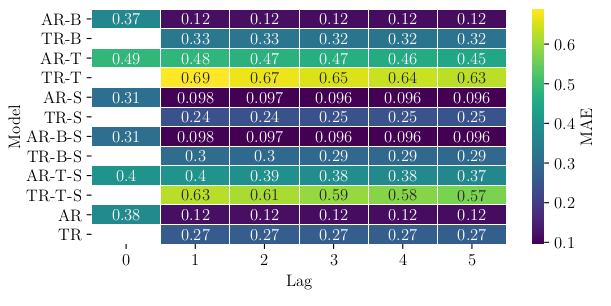
\includegraphics{python_figs/heat_ar_model_score.png} %\textbf{same colormap as MAE or obly for grids} 
    \caption{Heatmap showing the the performance of AR models. \textbf{This is currently only based on four pixels. Update the data}}
    \label{fig:results_ar_models}
\end{figure}
% se ark + flytt over bilde 
Figure \ref{fig:grid_mse_best_model} show the score of each pixel in the best model, \textbf{name best model}. Despite the fact that the pixel have no information about their neigbours, the model seem to grasp tha spatial relation . The patteren in figure, show clear distingstion between land and ocean and is far away from random noise wich was one of my conserns. 

The areas of the coast of Africa, Mediterranean ocean and the
The mountains areas light up as easier to predict. \textbf{Check if these are on average more cloudy.}

Table \ref{tab:weights_best_model} provide the statisics of the weights in this model. \textbf{comment if there is a large spread in the statistics.} \textbf{Do the pixels show a agreement in the relation between the input variables and cloud cover.}
\begin{figure}
    \centering
    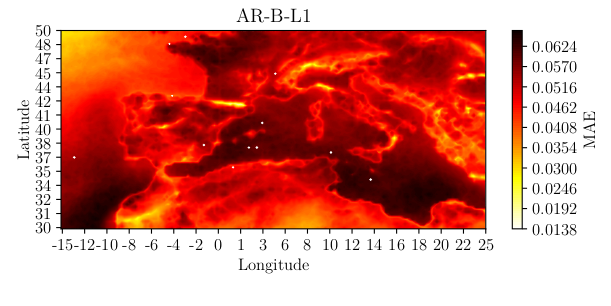
\includegraphics{python_figs/mea_best_ar_model_tcc.png}
    \caption{Grid showing the best models performance for all individual pixels. \textbf{Antar at hullene tettes når det gjelder den ordentlige beste modelen.} \textbf{This figure shows the mean, this will be updated with }}
    \label{fig:grid_mse_best_model}
\end{figure}

\begin{figure}
    \centering
    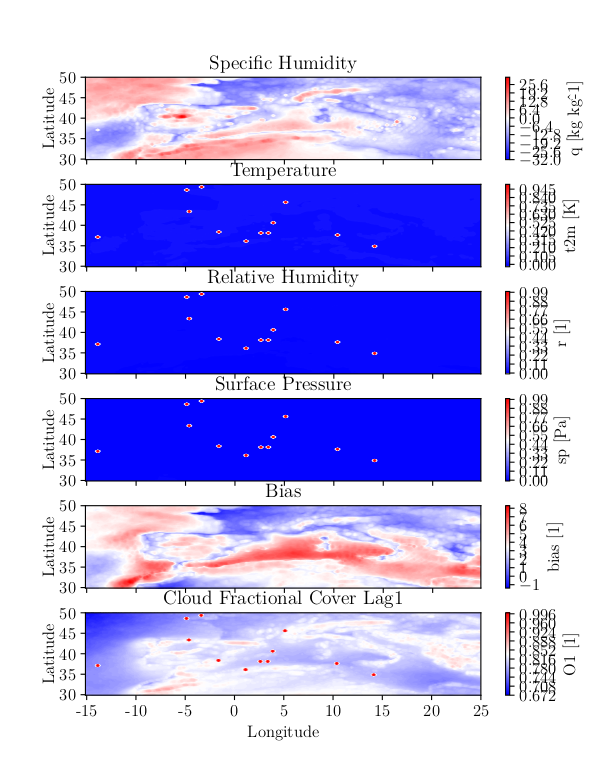
\includegraphics{python_figs/weights_best_ar_model.png}
    \caption{Update the statistics of the best AR-model.}
    \label{tab:weights_best_model}
\end{figure}

\clearpage

\subsection{Convolutional LSTM (ConvLSTM)}
The formulation of the air quality forecasting problem presented by \citeauthor{SunAirLSTM} is similar to the formulation of the cloud fractional cover forecasting problem presented in this study. 
%The machine learning experimental setup is adopted from the paper \citepaper{SunAirLSTM}.
% Endrer på arkitekturen - denne bruker -train - validation - test, en hvis prosentandel a

%\textbf{Below sentence is duplicated}
%Architectural decisions %such as batch size, sequence length, number of filters and number of layers 
%can cause the \acrshort{gpu} to run out of memory, resulting in non-trainable models.
%In these cases the compiled model is not trainable. 
To circumvent related issues, the \acrshort{convlstm}-models in this study was tuned manually. \textit{In this work, we have not explored the full range of possibilities that "ConvLSTM" potensially enables}. The list of hyperparameter is long when working with \acrshort{convlstm}-model. In the experiments conducted in this study a subset of them is tuned and the rest is kept constant.

The following section describe the tuned hyperparameters. The dataset is partitioned into subsets called batches. The batch size is the number of sequences a weight update is based on. Epochs describes the number of times the model loops over the entire dataset. The sequence length is the number of timestamps a model is optimized to learn to predict. Number of hidden states it the number of filters it learns in each layer, see Section \ref{sec:convolutional neural network} for a detailed description of hidden states. 
The filter size determines the number of neighbours influencing an activation. Using kernel 1x1 results in the state-to-state transitions similar to \acrshort{ar}-models by removing interactions between adjacent pixels. A more detailed description on these parameters is provided in Sections \ref{sec:convolutional neural network} to \ref{sec:convolutional_lstm}. 

This section describe the hyperparameters kept constant. Between each \acrshort{convlstm}-layer there is a \acrfull{batchnorm} layer, implemented using default settings. \textbf{Used on convolutional layers in this paper, but reccurent nets usually have the issuses its ment to handle. This has three major benefits, the network becomes less sensitive to the learning rate and weight initialization and it doesnt need dropout, the last accelerate the training proses}s (\cite{ioffe2015batch}).  ``Padding same'' is applied to all \acrshort{convlstm}-layer, to make sure the input and output dimensions are the same, see Section \ref{sec:padding}. The model returns a sequence and the input sequences are not shuffled. The output filter and kernel size is one to concatenate all the previous hidden states to one without altering the output dimension. This is necessary to predict a sequence of cloud fractional covers. 

The weights were initialized based on the scheme ``LeCun uniform'', see the paper for more descriptions (\cite{Lecun98efficientbackprop}). Callbacks such as %early stopping was impleme with patience \textbf{forgot to apply this when rerunning the models..} of 10 epochs and 
terminate on NaN's have been applied to avoid prolonged training time. The optimizer ADAM is used with the following settings, $\text{learning rate}=0.001$, $\text{beta1}=0.9$, $\text{beta2}=0.999$, $\text{epsilon}=1e-07$ (\cite{Kingma2015Adam:Optimization}). The default settings in Tensorflow use $\text{epsilon}=1e-08$. The loss function is \acrfull{mse}, and the models are evaluate based on \acrfull{mae}.
Both functions are described in more detail in Section \ref{sec:metrics}. %The main difference between these functions is that \acrshort{mse} penalize points further away. This has its advantages in training the model, but makes it more difficult to interpret the results. The squared numbers in the range 0 to 1 shrink.

\subsubsection{Experimental setup (ConvLSTM)}
Models are given names based on an extension of the convention from \citepaper{precip_nowcasting}.
% Trenge kanskje ikke nevne hva de hadde..?
By including batch size and sequence length %to $ConvLSTM-\text{hidden states}-filter$\times$filter$, 
the resulting naming convention becomes  $ConvLSTM-B_{x}-SL_{y}-\text{hidden states}-filter$\times$filter$. To clear any confusion Table \ref{tab:convlstm_config} provide a set of example configurations. \textbf{not random examples anymore, its all the models compiled in this study.}

\begin{table}[hp]
    \centering
    \resizebox{\textwidth}{!}{%
    \begin{tabular}{ccccc}
     \textbf{ConvLSTM Model} & \textbf{Sequence Length} & \textbf{Batch Size} & \textbf{Hidden States} & \textbf{Kernels} \\ \hline
    $B_{10}-SL_{24}-16-3\times3-16-3\times3$ & 24 & 10 & [16, 16]   & [3, 3] \\ \hline
    $B_{10}-SL_{24}-32-1\times1-32-1\times1$ & 24 & 10 & [32, 32]  & [1, 1] \\ \hline
    $B_{10}-SL_{24}-32-3\times3-32-3\times3$ & 24 & 10 & [32, 32] & [3, 3] \\ \hline
    $B_{10}-SL_{24}-32-5\times5-32-5\times5$ & 24 & 10 & [32, 32] & [5, 5] \\ \hline
    $B_{10}-SL_{24}-8-3\times3-8-3\times3-8-3\times3$ & 24 & 10 & [8, 8, 8] & [3, 3, 3] \\ \hline
    $B_{5}-SL_{6}-32-3\times3-32-3\times3-32-3\times3$ & 6 & 5 & [32, 32, 32] & [3, 3, 3] \\ \hline
    \end{tabular}%
    }
    \caption{Examples of \acrshort{conv}-model names and their configurations.}
    \label{tab:convlstm_config}
\end{table}
%\subsubsection{}
\begin{figure}
    \centering
    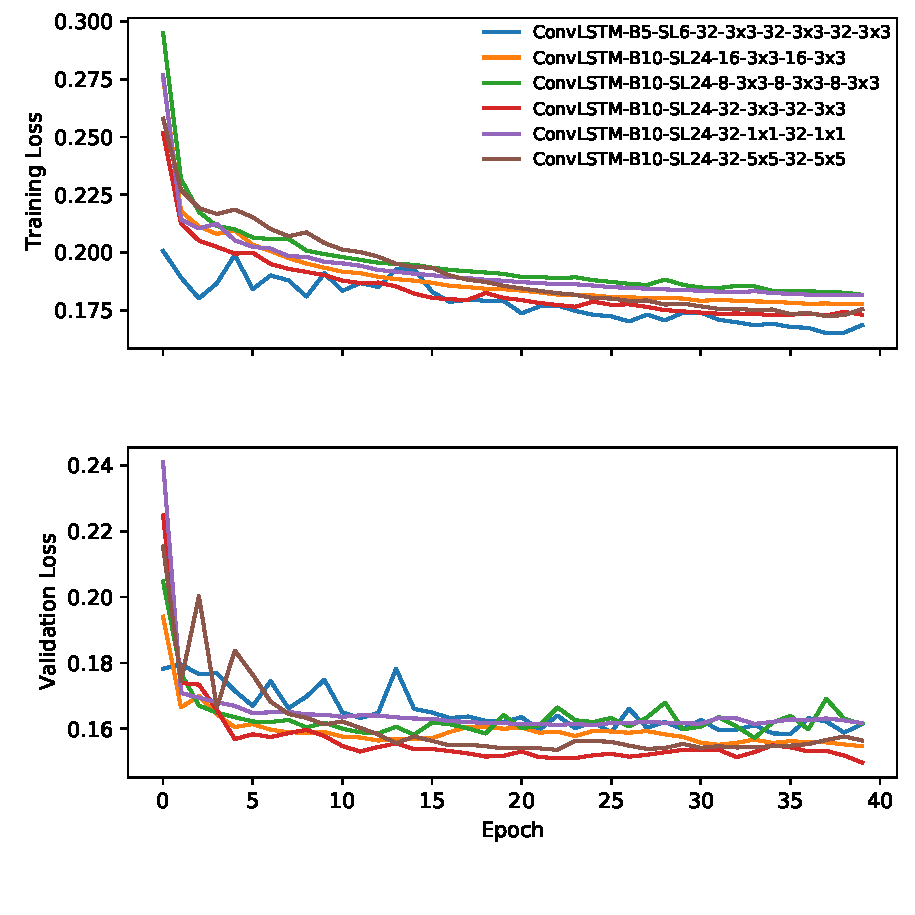
\includegraphics{python_figs/epoch_vs_loss.pdf}
    \caption{The loss for the trained model against epochs.}
    \label{fig:convlstm_loss}
\end{figure}
Figure \ref{fig:convlstm_loss} show the loss curves in the training process for all the compiled models in this study. They all ``learn'' the most in the first epoch, this is visible in the largest drop in loss moving from the first to second epoch. Note that the training loss is higher than the validation loss since there is a higher number of samples in this set and the loss is not scaled by the number of samples. 

Another means to further increase performance of train deeper models is to reduce the spatial or temporal resolution. This will reduce the noise in the input data, and the number of trainable parameters in the model. This trick was applied in \citepaper{precip_nowcasting}, they reduced the grid from $300\times300$ to $100\times100$ pixels. This is arguably not applicable for this task, since cloud cover has an average lifetime of one hour, as mentioned in Section \ref{sec:cloud_in_climate_system}. If applied it would most likely produce a significant loss of information.
%%%%%%%%%%%%%%%%%%%%%%%%% The copied dictionary is the result from tf.evaluate. 
\begin{table}[]
    \centering
    \resizebox{\textwidth}{!}{
    \begin{tabular}{c|lccc}
    \textbf{ConvLSTM Model} & \textbf{Train Loss} & \textbf{Val Loss} & \textbf{Test Loss} & \textbf{Num. Params.} \\ \hline 
    $B_{10}-SL_{24}-16-3\times3-16-3\times3$ & 0.1779 & 0.1547 & 0.1575 &  30 296\\ \hline
    % {"loss": 0.15752051770687103, "mean_squared_error": 0.15752056241035461, "r2_keras": 0.15506696701049805, "mean_absolute_error": 0.34570422768592834}

    $B_{10}-SL_{24}-32-1\times1-32-1\times1$ & 0.1817 & 0.1617 & 0.1649 & 13 464 \\ \hline
    % {"loss": 0.1649022251367569, "mean_squared_error": 0.1649022400379181, "r2_keras": 0.1159096509218216, "mean_absolute_error": 0.35085538029670715}
    \rowcolor{red!30}
    $B_{10}-SL_{24}-32-3\times3-32-3\times3$ & 0.1731 & 0.1497 & 0.1534 & 115 864 \\ \hline
    %{"loss": 0.15340088307857513, "mean_squared_error": 0.15340085327625275, "r2_keras": 0.17754235863685608, "mean_absolute_error": 0.33814743161201477}
    
    $B_{10}-SL_{24}-32-5\times5-32-5\times5$ & 0.1755 & 0.1564 & 0.1589 & 320 664 \\ \hline
    % {"loss": 0.15889282524585724, "mean_squared_error": 0.15889279544353485, "r2_keras": 0.147248774766922, "mean_absolute_error": 0.34079509973526}
    
    $B_{10}-SL_{24}-8-3\times3-8-3\times3-8-3\times3$ &  0.1817 & 0.1615 & 0.1634 & 12 920 \\ \hline
    % {"loss": 0.16335555911064148, "mean_squared_error": 0.16335561871528625, "r2_keras": 0.12448494136333466, "mean_absolute_error": 0.3477591276168823}
    
    $B_{5}-SL_{6}-32-3\times3-32-3\times3-32-3\times3$ & 0.1686 & 0.1615  & 0.1633 &  189 848 \\ \hline
    %{"loss": 0.1632702797651291, "mean_squared_error": 0.16327014565467834, "r2_keras": 0.09565786272287369, "mean_absolute_error": 0.3411720395088196}
    
      \end{tabular}
    }
    \caption{Results, metrics and number of parameters for the trained models. The best model \acrshort{convlstm}-model is highlighted in light blue. The loss presented is averaged over on batch, this is the keras default. Since its only used to chose the best model, there is no reason to upscale the numbers.}
    \label{tab:convlstmLoss}
\end{table}

From Figure \ref{fig:convlstm_loss} and Table \ref{tab:convlstmLoss} (highlighted in blue) its clear that the best performing \acrshort{convlstm}-model is the $ConvLSTM-B_{10}-SL_{24}-32-3\times3-32-3 \times3$. It has the lowest test and validation loss after 40 epochs. One model $ConvLSTM-B_{5}-SL_{6}-32-3\times3-32-3 \times3-32-3 \times3$ had a better training loss. As you can see based on the names it has a similar architecture, but an additional layer, this may have allowed it to learn a better representation on the training data presented, however the models are evaluated on unseen data and $ConvLSTM-B_{10}-SL_{24}-32-3\times3-32-3 \times3$ goes out winning.

$ConvLSTM-B_{10}-SL_{24}-32-3\times3-32-3 \times3$-model architecture is shown in Figure \ref{fig:best_ml_architecture}. The model consist of three \acrshort{batchnorm}  and  \acrshort{convlstm}-layer pairs. Both \acrshort{convlstm} layer have 32 hidden states and a $3\times 3$ kernel. The output layer has one hidden state and the kernel dimension of $1\times 1$. The input shape is $10\times24\times81\times161\times4$ and output $24\times81\times161\times1$. 
\begin{figure}
    \centering
    \begin{tikzpicture}[x={(1,0)},y={(0,1)},z={({cos(60)},{sin(60)})},
font=\sffamily\small,scale=1.9] % 1.7 passer bra på siden.

\tikzset{circle dotted/.style={dash pattern=on .05mm off 2mm,
                                         line cap=round}}

%
% comment these out if you want to see where the axes point to
% \draw[-latex] (0,0,0) -- (3,0,0) node[below]{$x$};
% \draw[-latex] (0,0,0) -- (0,3,0) node[left]{$y$};
% \draw[-latex] (0,0,0) -- (0,0,3) node[below]{$z$};
% a plane
\tikzset{pics/fake box/.style args={% #1=color, #2=x dimension, #3=y dimension, #4=z dimension
#1 with dimensions #2 and #3 and #4}{
code={
\draw[teal,ultra thin,fill=#1]  (0,0,0) coordinate(-front-bottom-left) to
++ (0,#3,0) coordinate(-front-top-right) --++
(#2,0,0) coordinate(-front-top-right) --++ (0,-#3,0) 
coordinate(-front-bottom-right) -- cycle;
\draw[teal,ultra thin,fill=#1] (0,#3,0)  --++ 
 (0,0,#4) coordinate(-back-top-left) --++ (#2,0,0) 
 coordinate(-back-top-right) --++ (0,0,-#4)  -- cycle;
\draw[teal,ultra thin,fill=#1!80!black] (#2,0,0) --++ (0,0,#4) coordinate(-back-bottom-right)
--++ (0,#3,0) --++ (0,0,-#4) -- cycle;
\path[teal,decorate,decoration={text effects along path,text={BATCH NORM}}] (#2/2,{3.4+(#3-2)/2},0) -- (#2/2,0,0);
}
}}
%3.0/1.5, 3.0/3.3, 3.0/5.0
\foreach \X / \Y in {3.0/1.3, 3.0/3., 3.0/4.6} 
%2.2,2.2,2.0
{
\draw pic (box1-\Y) at (\Y,-\X/2,0) {fake box=white!70!teal with dimensions 0.5 and {2*\X} and 1*\X};
}

%%%%%%%%%%%%%%%%%%%%%%%%%%%%%%%%%%%% 
\tikzset{pics/fake box/.style args={% #1=color, #2=x dimension, #3=y dimension, #4=z dimension
#1 with dimensions #2 and #3 and #4}{
code={
\draw[gray,ultra thin,fill=#1]  (0,0,0) coordinate(-front-bottom-left) to
++ (0,#3,0) coordinate(-front-top-right) --++
(#2,0,0) coordinate(-front-top-right) --++ (0,-#3,0) 
coordinate(-front-bottom-right) -- cycle;
\draw[gray,ultra thin,fill=#1] (0,#3,0)  --++ 
 (0,0,#4) coordinate(-back-top-left) --++ (#2,0,0) 
 coordinate(-back-top-right) --++ (0,0,-#4)  -- cycle;
\draw[gray,ultra thin,fill=#1!80!black] (#2,0,0) --++ (0,0,#4) coordinate(-back-bottom-right)
--++ (0,#3,0) --++ (0,0,-#4) -- cycle;
\path[gray,decorate,decoration={text effects along path,text={CONV LSTM}}] (#2/2,{3.4+(#3-2)/2},0) -- (#2/2,0,0);
}
}}

%%%%%%%%%%%%%%%%%%%%%%%%%%%%%%
\foreach \X / \Y in {3.0/1.6, 3.0/3.3, 3.0/4.9}
%2.2,2.2,2.0
{
\draw pic (box1-\Y) at (\Y,-\X/2,0) {fake box=white!70!gray with dimensions 0.5 and {2*\X} and 1*\X};
}

%\foreach \X/\Col in {0.0/red,0.2/green,0.4/cyan, 0.6/yellow, 6.8/blue} %{6.5/red,6.7/green,6.9/blue}
%{\draw[canvas is yz plane at x = \X, transform shape, draw = black, fill = \Col!50!white, opacity = 0.5] (0,0.5) rectangle (2,-1.5);}

%\draw[gray!60,thick] (-0.1,-0.1,-1.6) coordinate (1-1) -- (-0.1,-0.1,0.6) coordinate (1-2) -- (-0.1, 2.,0.6) coordinate (1-3) -- (-0.1, 2.1,-1.6) coordinate (1-4) -- cycle;
%\draw[gray!60,thick] (0.8,-0.1,-1.6) coordinate (2-1) -- (0.8,-0.1,0.6) coordinate (2-2) -- (0.8, 2.,0.6) coordinate (2-3) -- (0.8,2.1,-1.6) coordinate (2-4) -- cycle;

%%%%%%%%%%%%%%%%%%%%%%%%%%%%%%%%%%%% 
\tikzset{pics/fake box/.style args={% #1=color, #2=x dimension, #3=y dimension, #4=z dimension
#1 with dimensions #2 and #3 and #4}{
code={
\draw[gray,ultra thin,fill=#1]  (0,0,0) coordinate(-front-bottom-left) to
++ (0,#3,0) coordinate(-front-top-right) --++
(#2,0,0) coordinate(-front-top-right) --++ (0,-#3,0) 
coordinate(-front-bottom-right) -- cycle;
\draw[gray,ultra thin,fill=#1] (0,#3,0)  --++ 
 (0,0,#4) coordinate(-back-top-left) --++ (#2,0,0) 
 coordinate(-back-top-right) --++ (0,0,-#4)  -- cycle;
\draw[gray,ultra thin,fill=#1!80!black] (#2,0,0) --++ (0,0,#4) coordinate(-back-bottom-right)
--++ (0,#3,0) --++ (0,0,-#4) -- cycle;
\path[gray,decorate,decoration={text effects along path,text={INPUT}}] (#2/2,{2.4+(#3-2)/2},0) -- (#2/2,0,0);
}
}}

%%%%%%%%%%%%%%%%%%%%%%%%%%%%%%
\foreach \X / \Y in {3.0/-1.0}
%2.2,2.2,2.0
{
\draw pic (box1-\Y) at (\Y,-\X/2,0) {fake box=white!70!green with dimensions 2.5 and {2*\X} and 1*\X};
}

\tikzset{pics/fake box/.style args={% #1=color, #2=x dimension, #3=y dimension, #4=z dimension
#1 with dimensions #2 and #3 and #4}{
code={
\draw[gray,ultra thin,fill=#1]  (0,0,0) coordinate(-front-bottom-left) to
++ (0,#3,0) coordinate(-front-top-right) --++
(#2,0,0) coordinate(-front-top-right) --++ (0,-#3,0) 
coordinate(-front-bottom-right) -- cycle;
\draw[gray,ultra thin,fill=#1] (0,#3,0)  --++ 
 (0,0,#4) coordinate(-back-top-left) --++ (#2,0,0) 
 coordinate(-back-top-right) --++ (0,0,-#4)  -- cycle;
\draw[gray,ultra thin,fill=#1!80!black] (#2,0,0) --++ (0,0,#4) coordinate(-back-bottom-right)
--++ (0,#3,0) --++ (0,0,-#4) -- cycle;
\path[gray,decorate,decoration={text effects along path,text={OUTPUT}}] (#2/2,{2.6+(#3-2)/2},0) -- (#2/2,0,0);
}
}}

\foreach \X / \Y in {3.0/6.1}
%2.2,2.2,2.0
{
\draw pic (box1-\Y) at (\Y,-\X/2,0) {fake box=white!70!blue with dimensions 1.0 and {2*\X} and 1*\X};
}

%\foreach \X in {4,1,3}
%{\draw[gray!60,thick] (1-\X) -- (2-\X);}

\node[draw,single arrow, orange,fill=orange!30] at (0.8, 0.5,0) {BATCH};
\node[draw,single arrow, orange,fill=orange!30] at (2.4, 0.5,0) {$3\times 3$};
\node[draw,single arrow, orange,fill=orange!30] at (4., 0.5,0) {$3\times 3$};
\node[draw,single arrow, orange,fill=orange!30] at (5.6, 0.5,0) {$1\times 1$};

%\begin{scope}[on background layer]
%\node[orange,thick,rounded corners,fill=orange!30,fit=(A1) (A3)]{};
%\node[gray,thick,rounded corners,fill=gray!10,fit=(B1) (B3)]{};
%\end{scope}

%\foreach \X in {1,2,3}
%{\draw[-latex] (A\X) -- (B2);}

\draw[thick](0.2, 3.3)node[scale=1.]{\small $10\times 24\times 81\times 161 \times 4 $};
\draw[thick](1.5, -2)node[scale=1.]{\small $10\times 24\times81\times 161 \times 32 $};
\draw[thick](3.8, 3.3)node[scale=1.]{\small $10\times 24\times 81\times 161 \times 32 $};
\draw[thick](5.0, -2)node[scale=1.]{\small $10\times 24\times 81\times 161 \times 1 $};
\draw[thick](6.6, 3.3)node[scale=1.]{\small $10\times 24\times 81\times 161 \times 1 $};
\end{tikzpicture}
    \caption{The architecture of the cloud cover forecasting model developed in this study. }
    \label{fig:best_ml_architecture}
\end{figure}
In this input volume is simplified as a green box. One batch, of the detailed 5-dimensional input volume is displayed in Figure \ref{fig:input_volume_conv_lstm}. One batch (green box), consist of a batch size number of sequences, here 10. A sequence is composed of a sequence length, of here 24, hourly weather data volumes of $81\time161\times4$-dimensions.
\begin{figure}
    \centering
    %
\tikzset{every picture/.append style={scale=1.0}}
\begin{tikzpicture}[x={(1,0)},y={(0,1)}, z={({cos(60)},{sin(60)})},
font=\sffamily\small, scale=1.0]

\tikzset{pics/fake box/.style args={% #1=color, #2=x dimension, #3=y dimension, #4=z dimension
#1 with dimensions #2 and #3 and #4}{
code={
\draw[teal,ultra thin,fill=#1,opacity=0.25]  (0,0,0) coordinate(-front-bottom-left) to
++ (0,#3,0) coordinate(-front-top-right) --++
(#2,0,0) coordinate(-front-top-right) --++ (0,-#3,0) 
coordinate(-front-bottom-right) -- cycle;
\draw[teal,ultra thin,fill=#1, opacity=0.25] (0,#3,0)  --++ 
 (0,0,#4) coordinate(-back-top-left) --++ (#2,0,0) 
 coordinate(-back-top-right) --++ (0,0,-#4)  -- cycle;
\draw[teal,ultra thin,fill=#1!80!black, opacity=0.25] (#2,0,0) --++ (0,0,#4) coordinate(-back-bottom-right)
--++ (0,#3,0) --++ (0,0,-#4) -- cycle;
\path[teal,decorate,decoration={text effects along path,text={}}] (#2/2,{3.4+(#3-2)/2},0) -- (#2/2,0,0);
}
}}

%%%%%%%%%% Green box in the back symbolizing batches 
\foreach \X / \Y in {2.3/-1.5} {
\draw pic (box1-\Y) at (\Y,-\X/,0) {fake box=green with dimensions 14.6 and {2*\X} and 1*\X};
}


%%%%%%%%%%%%%%%%%%%%%%%%%%%%%% BLUE BOX
\foreach \X / \Y in {1.5/-1.0, 1.5/6} {
\draw pic (box1-\Y) at (\Y,-\X/,0) {fake box=white!25!cyan with dimensions 6.9 and {2*\X} and 1*\X};
}


%%%%%%%%%%%%%%%%%%%%%%%%%%%%%%% Weather data volume 1.
\foreach \X/\Col in {0.0/red, 0.2/green, 0.4/cyan, 0.6/yellow} %{6.5/red,6.7/green,6.9/blue}
{\draw[canvas is yz plane at x = \X, transform shape, draw = black, fill = \Col!50!white, opacity = 0.5] (0,0.5) rectangle (2,-1.5);}

%\draw[gray!60,thick] (-0.1,-0.1,-1.6) coordinate (1-1) -- (-0.1,-0.1,0.6) coordinate (1-2) -- (-0.1, 2.,0.6) coordinate (1-3) -- (-0.1, 2.1,-1.6) coordinate (1-4) -- cycle;

%\draw[gray!60,thick] (0.8,-0.1,-1.6) coordinate (2-1) -- (0.8,-0.1,0.6) coordinate (2-2) -- (0.8, 2.,0.6) coordinate (2-3) -- (0.8,2.1,-1.6) coordinate (2-4) -- cycle;

%\foreach \X in {4,1,3}{\draw[gray!60,thick] (1-\X) -- (2-\X);}

\tikzset{pics/fake box/.style args={% #1=color, #2=x dimension, #3=y dimension, #4=z dimension
#1 with dimensions #2 and #3 and #4}{
code={
\draw[teal,ultra thin]  (0,0,0) coordinate(-front-bottom-left) to
++ (0,#3,0) coordinate(-front-top-right) --++
(#2,0,0) coordinate(-front-top-right) --++ (0,-#3,0) 
coordinate(-front-bottom-right) -- cycle;
\draw[teal,ultra thin] (0,#3,0)  --++ 
 (0,0,#4) coordinate(-back-top-left) --++ (#2,0,0) 
 coordinate(-back-top-right) --++ (0,0,-#4)  -- cycle;
\draw[teal,ultra thin,fill=#1!80!black] (#2,0,0) --++ (0,0,#4) coordinate(-back-bottom-right)
--++ (0,#3,0) --++ (0,0,-#4) -- cycle;
\path[teal,decorate,decoration={text effects along path,text={}}] (#2/2,{3.4+(#3-2)/2},0) -- (#2/2,0,0);
}
}}

%%%%%%%%%%%%%%%%%%%%%%%%%%%%%%%%%%%%%%%%%%%%

%%%%%%%%%%%%%%%%%%%%%%%%%%%%%% BLUE BOX

\foreach \X/\Col in {2.0/red,2.2/green,2.4/cyan, 2.6/yellow} %{6.5/red,6.7/green,6.9/blue}
{\draw[canvas is yz plane at x = \X, transform shape, draw = black, fill = \Col!50!white, opacity = 0.5] (0,0.5) rectangle (2,-1.5);}

\foreach \X/\Col in {5.0/red,5.2/green,5.4/cyan, 5.6/yellow} %{6.5/red,6.7/green,6.9/blue}
{\draw[canvas is yz plane at x = \X, transform shape, draw = black, fill = \Col!50!white, opacity = 0.5] (0,0.5) rectangle (2,-1.5);}

%%%%%%%%%%%%%%% Second bow
\foreach \X/\Col in {7.0/red,7.2/green,7.4/cyan, 7.6/yellow} %{6.5/red,6.7/green,6.9/blue}
{\draw[canvas is yz plane at x = \X, transform shape, draw = black, fill = \Col!50!white, opacity = 0.5] (0,0.5) rectangle (2,-1.5);}

\foreach \X/\Col in {9.0/red,9.2/green,9.4/cyan, 9.6/yellow} %{6.5/red,6.7/green,6.9/blue}
{\draw[canvas is yz plane at x = \X, transform shape, draw = black, fill = \Col!50!white, opacity = 0.5] (0,0.5) rectangle (2,-1.5);}

\foreach \X/\Col in {12.0/red,12.2/green,12.4/cyan, 12.6/yellow} %{6.5/red,6.7/green,6.9/blue}
{\draw[canvas is yz plane at x = \X, transform shape, draw = black, fill = \Col!50!white, opacity = 0.5] (0,0.5) rectangle (2,-1.5);}

%%%%%%%%%%%%%%%%%%% ADDING TEXT
\node[color = gray, thick] at (6, 3.3) {\Large Batch \#0};
\node[color = blue!60, thick] at (1.0, -2.0) {\large SEQUENCE \#0};
\node[color = blue!60, thick] at (8.0, -2.0) {\large SEQUENCE \#1};
\node[color = gray, thick, rotate=60] at (0.3, 0.1) {$00:00$};
\node[color = gray, thick, rotate=60] at (2.3, 0.05) {$01:00$};
\node[color = gray, thick, rotate=60] at (5.3, 0.0) {$23:00$};

\node[color = gray, thick, rotate=60] at (7.3, 0.1) {$00:00$};
\node[color = gray, thick, rotate=60] at (9.3, 0.05) {$01:00$};
\node[color = gray, thick, rotate=60] at (12.3, 0.0) {$23:00$};


%%%%%%%%%%%%%% Dotted lines
\path[draw, thick, dotted] (3.0, 0.5) edge (4., 0.5);
\path[draw, thick, dotted] (10.0, 0.5) edge (11., 0.5);

\end{tikzpicture}
%\end{document}

    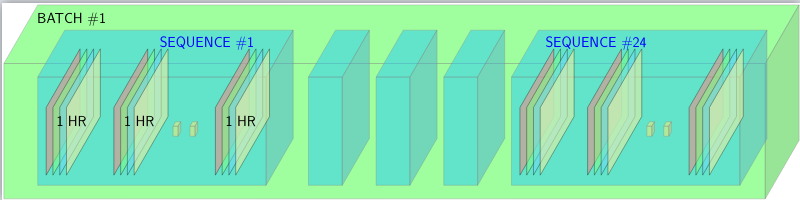
\includegraphics[scale=0.6]{ChapterX_Results_and_Conclusion/computational_experiments/temp_input_volume.png}
    \caption{Illustration of the content of the first batch. A batch is a 5-dimensional data volume. For each hour the weather data volume is $81\times 161\times 4$, a sequence consist of 24 of these volumes and a batch contain 10 sequences. \ref{fig:best_ml_architecture} \textbf{Comment to Trude, I have drawn this in tikz in a seperate overleaf doc, due to some scaling issues I've used the screenshot to by some time.}}
    \label{fig:input_volume_conv_lstm}
\end{figure}

The $ConvLSTM-B_{10}-SL_{24}-32-1\times1-32-1 \times1$-model is trained without allowing knowledge trasfer between neigbours. This is the architecture is the most similar \acrshort{ar}-models. From Table \ref{tab:convlstmLoss} you can see it has the worst Test loss among the trained models. This indicate that information from adjasent pixels is usefull. Its necesarry to mention that there is a significant difference between a \acrshort{ar}-model and a \acrshort{convlstm}-model with $1\times 1$ kernel and that is that the \acrshort{ar}-model train a different weight in all pixels, while the \acrshort{convlstm}-model utilize the same weights over the entire grid. 
%Not suprising ths that the number of parameters increase as the kernel increasse. 
\clearpage

\subsection{Local/Gridded Performance}
%\textbf{Pga. drop remainder batch num samples of MAE is 43 680 vs 43 824 in others}
%%%%%%%%%%%%%%%%%%%%%%%%%%%%%%%%%%%%%%% Commenting on spatial patterens
\begin{figure}
    \centering
    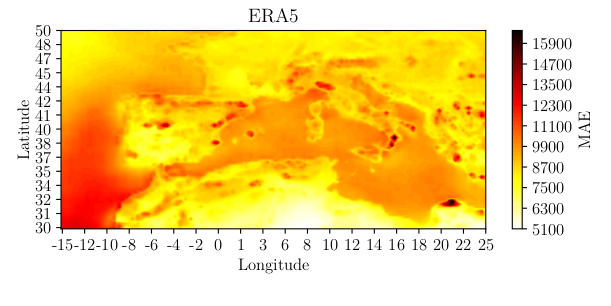
\includegraphics{python_figs/mae_era_vs_target_test_period_2014_to_2018.png}
    \caption{MAE between ERA5 and \acrshort{ecc} in the period from 01.01.2014 to 31.12.2018.}
    \label{fig:MAE_era}
\end{figure}
Figure \ref{fig:mae_era_target} show the \acrshort{mae} between the \acrshort{cfc} in ERA5 and \acrshort{ecc}. It reveals systematic errors over the Mediterranean Sea and in the Atlantic Ocean of the coast of Gibraltar. Mountainous areas in the French and Italian Apls
among other light up, revealing that they are predicted \textbf{skill er et bedre ord}. 


Figure \ref{fig:MAE_convlstm} show the performance of the best convolutional model in the period 2014-2018, the period is in fact a few hours shorter, since the models ran with ``drop remainder batch''. Both these representations of \acrshort{cfc} have trouble with the Nile Delta. This doesn't not seem to be the case for \textbf{update:the best ar model}.
\begin{figure}
    \centering
    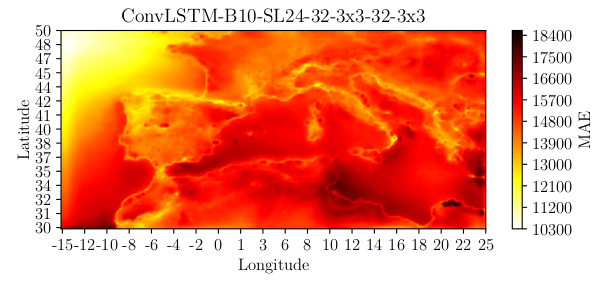
\includegraphics{python_figs/mae_convlstm_vs_target_test_period_2014_to_2018.png}
    \caption{MAE ConvLTSM for the test period, pga. drop batch reminder the number of samples generating the foundaion for this plot is 43 680, \textbf{the era5 plot is currently 43 824, I'm considering reducing this so that they are equal. A a crucial factor is how simple it would be to do the same for ERA5} }
    \label{fig:MAE_convlstm}
\end{figure}

\begin{figure}
    \centering
    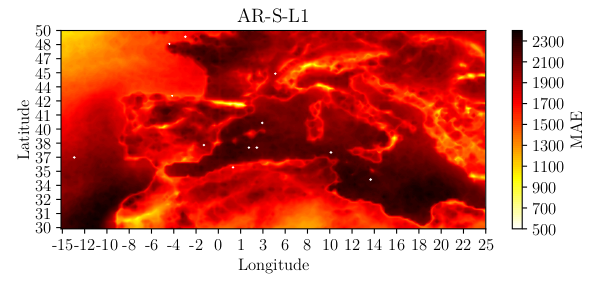
\includegraphics{python_figs/mea_best_ar_model_tcc_L1_in_folder_AR-S-L1.png}
    \caption{\textbf{Update to best AR model} Mistnker at det er noe feil med skaleringen her. Finner ikke feilen, beregningen er nanmean av test samples også skaleres det med antall test samples som er 43649 .. Num test samples er tilgjengelig i filen hvor performance er lagret...}
    \label{fig:MAE_AR}
\end{figure}

%%%%%%%%%%%%%%%%%%%%%%%%%%%%%%% Commenting on accumulated score 
Summing over all pixels results in a MAE of $1.16508643\cdot10^8$. These systematic errors appear to be in region fewer observation, i.e. mountainous regions and over the sea. %Dust storm causing the red ocean off the coast of Sahara..?
\begin{table}[]
    \centering
    \begin{tabular}{llll}
    \multicolumn{1}{c}{\textbf{}} & \textbf{ERA5} & \multicolumn{1}{c}{\textbf{AR}} & \multicolumn{1}{c}{\textbf{ConvLSTM}} \\ \hline
    MAE & $1.16508643\cdot10^8$ &  X & $1.91520128 \cdot 10^8$ 
    \end{tabular}
    \caption{Total \acrfull{mae} in the period ...}
    \label{tab:tot_mae_score}
\end{table}


\subsection{Visual comparison predicting sequence}
In this section provide a visual comparison of the \textbf{best} \acrshort{ar}-model, $ConvLSTM-B_{10}-SL_{24}-32-3\times3-32-3 \times3$-model, ERA5 and the target, \acrshort{cfc} in \acrshort{ECC}. Figure \ref{fig:target_predict_era5_horizontal} show the first of a series of four plots generated to illustrate a step by step comparison of the \acrshort{cfc}. The full series is shown in Appendix \ref{app:pred_sequence}. The series is 24 hours of January first 2014.

The similarity between \acrshort{ecc}, \acrshort{ar}, and ERA5 is impressive. They capture a similar spatial pattern, ERA5 is a 

the \acrshort{ecc} show a smoother version and the ERA5 have a higher fraction of cloud cover and sharper boundaries. 
%%%% TARGET PREDICITON ERA5
\begin{figure}[ht]
    \centering
    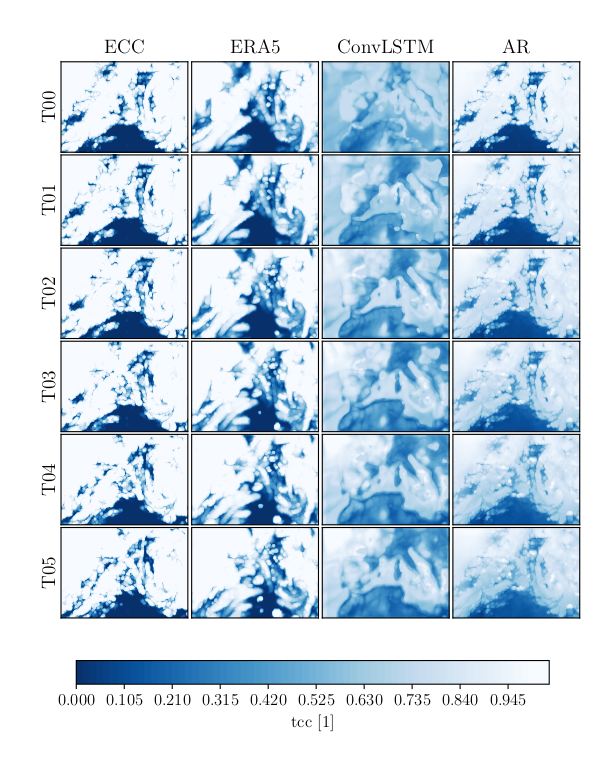
\includegraphics[sale=0.1]{python_figs/comparting_seq_part_1_of4.png}
    \caption{First of 4 part since the sequence is 24 hours long, the full series of plots for this sequence can be found in Appendix \ref{app:pred_sequence}.}
    \label{fig:target_predict_era5_horizontal}
\end{figure}
At first glance it clear that the \acrshort{convlstm}-model have learned which pixels are land and which is ocean. After a few hours its gets more distinct in its cloud cover and a weaker version of the triangle structure found in the three others begins to reveal itself. As the time pass by the cloud cover progress onto the continent and the \acrshort{convlstm} show signs of increased clod cover over parts of Spain and France.
The values are smoother and they are in this series are in the middle range.

\textbf{Comment on AR when its updated}
\textbf{sjekk appendix om det skjer noe som er ver å påpeke lenger ut i serien.}

The \acrshort{convlstm}-model is optimized to fit a sequence, while the \acrshort{ar}-model is optimized to fit the next timestep, not a sequence.
\textbf{Can you see this in Figure \ref{fig:target_predict_era5_horizontal} ..? Does the ar gradually become worse?}

\textbf{Run av med en oppsummerende setning om AR og ConvLSTM}
Is it evident that the \acrshort{convlstm} is better at predicting spatial patterns as expected or does it all resemble random noise. Is the predicted values in sample or out of sample.

The displayed sequence predicted by $ConvLSTM-B_{10}-SL_{24}-32-3\times3-32-3 \times3$-model contain no out of sample values. In total for the entire period of 2014-2018 $0.5\%$ is unphysical. The out-of-sample values predicted are purely on the negative sign, having a minimum at -1. 
%17140/3129840 = 0.005476318278250646

\textbf{Does AR ever predict out of sample values}
\textbf{Finn beste AR modell, prediker hele sekvensen, bergn MAE og tell ant. out of sample values}

\subsection{Summary} \label{sec:summary_num}
\textbf{Hva skal med}
\begin{itemize}
    \item 
\end{itemize}

Comparisons of inputdata to the works by \citeauthor{precip_nowcasting} (\citeyear{precip_nowcasting}) and \citeauthor{SunAirLSTM} (\citeyear{SunAirLSTM}), is done based on input volumes. %\textbf{Add the input volume}
The dimensions are flattened to generalize the comparison. \citepaper{precip_nowcasting} is trained on $1,629,600,000$ data points, \citepaper{SunAirLSTM} on $28,513,800$ and \acrshort{ecc} on $21,220,315,200$. The models in this study is trained on more than 10 times the amount of data. \textbf{Understrek at detter er en achievement siden er er vanskeligere å trene en model på mer data.}
% NOTES IN CASE I FORGET WHERE THE NUMBER CAME FROM
%\begin{enumerate}
%    \item Radar Echo: 1 sequence is 20 Frame one frame is 100x100. Train seq. 8148, 2037 for valid and 2037 for test. 
%    \item 1629600000 Num Train, 407400000 Num Valid and 407400000 num Test
%    \item KDD Weather data 21x31x5 365.25*24 (Train), 30*24(Valid, test)
%    \item 28513800 (Train) samples, 2343600 (Valid, Test)
%\end{enumerate}
%\textbf{Ønsker å understreke dette for det er }
It is more difficult to train a models on a larger amount of data. 



\clearpage
\section{Practical implications - OUTDATED} \label{sec:practical_implications}
It is necessary to have a understanding of the needs of the end product before conducting large machine learning projects. Answering questions like: What will it be used for and how can it be implemented in useful way?

A major downside of the data driven learning approach is the rigid resolution. A trained model can only be used on similar problems, with the same spatiotemporal resolution. For applications like climate models, output comes in a wide range of different resolutions. Before implementing the finished product in a new model of a different resolution, it would need to be retrained on the resolution of the climate model under development. This process involves both remapping of the dataset and retraining the model at the correct resolution. This is a time consuming process involving finding a new set of hyperparameters suitable for the new resolution. % It essentially means starting over.

Once trained on global climate datasets, machine learning models provide fast results even for complex parameterization which is what makes them suitable for the application of climate modelling. Most machine learning packages are developed using Python. \acrfull{esm} are implemented in python. Methods for including the trained parameterizations need to be developed.
 
\subsection{Any implications based on the results presented in this chapter.}